\documentclass[a4paper,11pt]{article}
\usepackage[latin1]{inputenc}
\usepackage[T1]{fontenc}
\usepackage{bbm}
\usepackage{amsmath}
\usepackage{indentfirst}
\usepackage{fullpage}
\usepackage{url}
\usepackage{graphicx}
\usepackage[center,footnotesize]{caption}
\usepackage[section]{placeins}
\usepackage{subfig}
\title{Series 5}
\date{October 18, 2011}
\author{Genomics and bioinformatics - Week 5}
\begin{document}
\maketitle

\section{Markow model}
Lorem ipsum.

\section{Reading frame}
In this exercise you are given an nucleotide sequence which contains a coding region somewhere. You have to deduce what is the reading frame of this coding region.

The general procedure to find the right frame for reading a nucleotide sequence is to convert the nucleotide sequence into the corresponding possible amnio acid sequences and see which one makes the most sense. As you know, the base pairs are read three by three and translated into amino acids. One can hence read a sequence in three different ways: A, B and C.

\begin{figure}[h!]
	\centering
	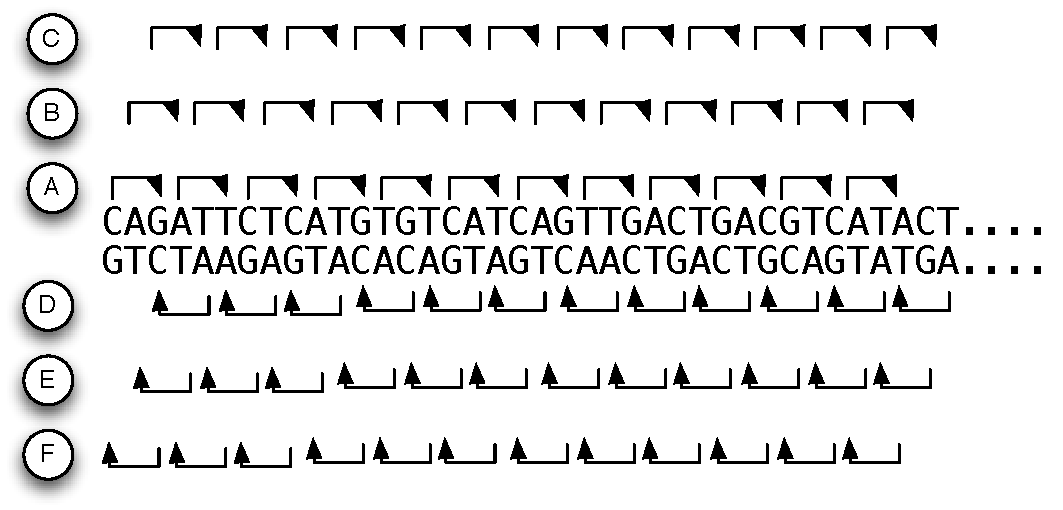
\includegraphics[width=1.0\textwidth]{reading_frame.pdf}
	\caption{Three possible reading frames.}
	\label{fig:gene_distribution_rib}
\end{figure}

So, to convert a base pair sequence (e.g. \texttt{CAGATTATG}...) to an amino acid sequence (e.g. \texttt{GWLPHLQRI}...) you cut the base pair sequence in pieces of 3 nucleotides (e.g. \texttt{"CAG", "ATT",...}), and use a conversion table that links any possible 3mer to one of the 21 amnio acids. For instance, \texttt{CAG} codes for glutamine.

\subsection{three-mers}
To build the conversion table that links 3-mers to amino acids. We first need to build an exhaustive list of three-mers. Write the function that takes four base pairs this as input and generates all the possible permutations of size three.

\begin{quote}
\begin{verbatim}
	def all_threemers(bases=['a','g','t','c']):
		...
\end{verbatim}
\end{quote}
	
The output should start like this and have 213 elements:

asdasddsa

\subsection{BP to AA}
We can now build the function the takes a three-mer as entry and outputs an amino acid. If you build the list correctly in the previous step the corresponding amino acids are the following:

\texttt{FFLLSSSSYY**CC*WLLLLPPPPHHQQRRRRIIIMTTTTNNKKSSRRVVVVAAAADDEEGGGG}

\subsection{Sequence to protein}
You can now write the function that takes a nucleotide sequence as entry and outputs a protein sequence.

\subsection{Sequence to protein}
You can now call the function you wrote in the last step with the three different possible frames and decide which one is right one.

\section{Blast}
Lorem ipsum.

\end{document}
